\documentclass{standalone}
\usepackage{tikz}
\usetikzlibrary{arrows,automata}
\usepackage[font=footnotesize,labelfont=bf]{caption}
\usepackage{pgf}
\usepackage[T1]{fontenc}

%% \author{Joshua Meyer}
%% \title{Some TikZ Examples}
%% \maketitle

%% \begin{document}
%% \begin{tikzpicture}[->,>=stealth',shorten >=1pt,auto,node distance=4cm,semithick]
    
%%     \node[state,initial,circle,minimum size=1.25cm]	(s1)		[]					{$1$};
%%     \node[state,accepting,circle,minimum size=1.25cm]	(s2)		[right of=s1]		{$2$};
 
%%     \path (s1) 	edge		[bend left] 	node {\texttt{pdf:word}} 			(s2);
%% \end{tikzpicture}
%% \end{document}


\begin{document}
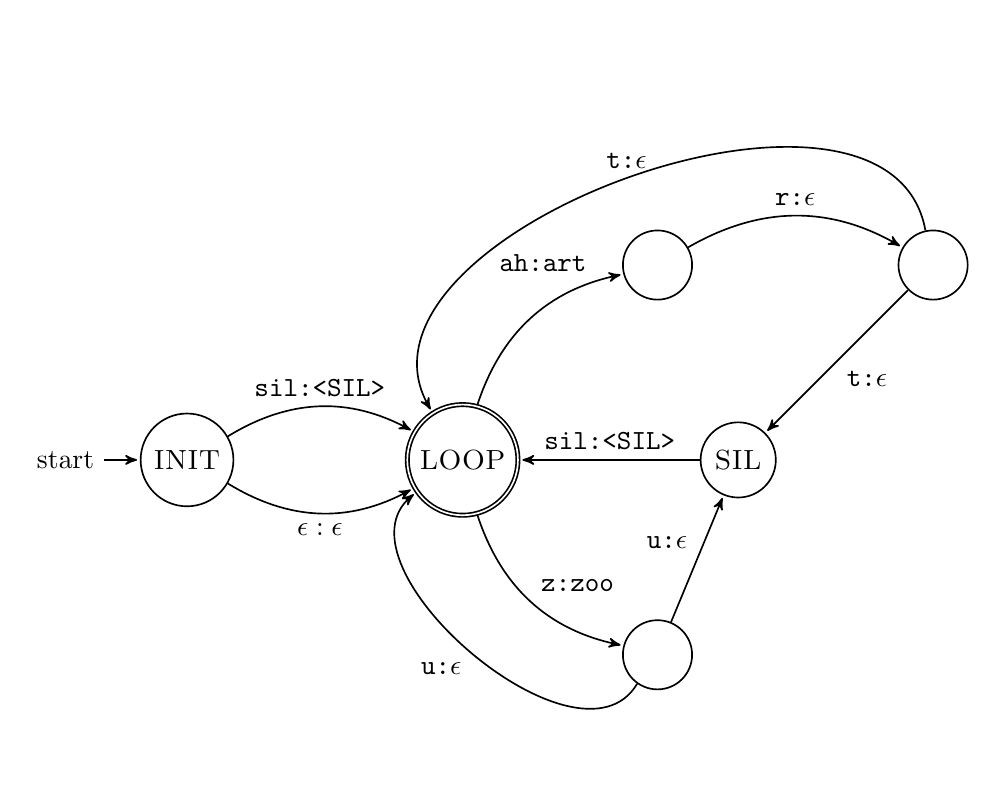
\begin{tikzpicture}[->,>=stealth',shorten >=1pt,auto,node distance=3.5cm,
                    semithick]
  \tikzstyle{every state}=[]

  \node[initial,state] (1)                    {\textsc{INIT}};
  \node[state,accepting]         (2) [right of=1]       {\textsc{LOOP}};

  \node[state]         (3) [above right of=2] {};
  \node[state]         (4) [right of=3]       {};

  \node[state]         (6) [below right of=2] {};

  \node[state]         (7) [right of=2]       {\textsc{SIL}};

  \path (1) edge [bend right=-30]  node {\texttt{sil:<SIL>}} (2)
            edge [bend right=30]   node [below] {$\epsilon:\epsilon$} (2)

        (2) edge [bend right=-30]      node [very near end]{ \texttt{ah:art} } (3)
        (3) edge [bend right=-30]      node { \texttt{r:$\epsilon$} } (4)
        (4) edge [bend left=-100]  node [above]{\texttt{t:$\epsilon$}} (2)
        (4) edge []  node {\texttt{t:$\epsilon$}} (7)

        (2) edge [bend right=30]      node{ \texttt{z:zoo} } (6)
        (6) edge [bend left=100]  node { \texttt{u:$\epsilon$}} (2)
        (6) edge []  node { \texttt{u:$\epsilon$}} (7)

        (7) edge []  node [above]{\texttt{sil:<SIL>}} (2);

\end{tikzpicture}
\end{document}

%% \begin{tikzpicture}[->,>=stealth',shorten >=1pt,auto,node distance=4cm,semithick]
    
%%     \node[state,initial,circle,minimum size=1.25cm]	(s1)		[]					{$1$};
%%     \node[state,accepting,circle,minimum size=1.25cm]	(s2)		[right of=s1]		{$2$};
 
%%     \path (s1) 	edge		[bend left] 	node {\texttt{phone:word}} 			(s2);
%% \end{tikzpicture}

%% \begin{center}	
%% \begin{tikzpicture}[->,>=stealth',shorten >=1pt,auto,node distance=2.8cm,semithick]
    
%%     \node[state, initial]	(s1)		[]					{$1$};
%%     \node[state,]			(s2)		[right of=s1]		{$2$};
%%     \node[state,accepting]	(s3)		[right of=s2]		{$3$};
 
%%     \path (s1) 	edge		[] 				node {a} 			(s2);
%%     \path (s2) 	edge		[loop above]		node {a} 			(s2);
%%     \path (s2)  edge    	[]     			node {$\epsilon$} 	(s3);
%%     \path (s3) 	edge		[loop right] 	node {b} 			(s3);
    
%% \end{tikzpicture}
%% \captionof{figure}{\texttt{L.fst}}
%% \label{tikz}
%% \end{center}





%% \begin{center}
%% \begin{tikzpicture}[->,>=stealth',shorten >=1pt,auto,node distance=2.8cm,semithick]
    
%%     \node[state, initial]	(s1)		[]					{$1$};
%%     \node[state,]			(s2)		[right of=s1]		{$2$};
%%     \node[state,accepting]	(s3)		[right of=s2]		{$3$};
%%     \node[state,]			(s4)		[below right of=s2]	{$4$};
 
%%     \path (s1) 	edge		[] 				node {a} 	(s2);
%%     \path (s2) 	edge		[bend left]		node {b} 	(s3);
%%     \path (s2)  edge    	[bend right]     node {b}     (s4);
%%     \path (s3) 	edge		[bend left] 		node {a} 	(s2);
%%     \path (s4) 	edge		[bend right] 	node {a} 	(s3);
    
%% \end{tikzpicture}
%% \end{center}


%% \begin{center}
%% \begin{tikzpicture}[->,>=stealth',shorten >=1pt,auto,node distance=2.8cm,semithick]
    
%%     \node[state, initial]	(s1)		[]					{$1$};
%%     \node[state,]			(s2)		[right of=s1]		{$2$};
%%     \node[state,accepting]	(s3)		[right of=s2]		{$3$};
%%     \node[state,accepting]	(s4)		[below right of=s2]	{$4$};
 
%%     \path (s1) 	edge		[] 				node {a} 	(s2);
%%     \path (s2) 	edge		[bend left]		node {b} 	(s3);
%%     \path (s3) 	edge		[bend right] 	node {a} 	(s4);
%%     \path (s4) 	edge		[bend left] 		node {a} 	(s2);
%%     \path (s4) 	edge		[bend right] 	node {b} 	(s3);

%% \end{tikzpicture}
%% \end{center}



%% \begin{center}
%% \begin{tikzpicture}[->,>=stealth',shorten >=1pt,auto,node distance=2.8cm,semithick]
    
%%     \node[state, initial]	(s1)		[]					{$1$};
%%     \node[state,]			(s2)		[right of=s1]		{$2$};
%%     \node[state,accepting]	(s3)		[right of=s2]		{$3$};
%%     \node[state,]			(s4)		[below right of=s1]	{$4$};
%%     \node[state,]			(s5)		[below left of=s3]	{$5$};

%%     \path (s1) 	edge		[loop above] 	node {a} 	(s1);
%%     \path (s1) 	edge		[] 				node {b} 	(s2);
%%     \path (s1) 	edge		[bend right] 		node {b} 	(s4);

%%     \path (s2) 	edge		[]				node {a} 	(s3);
%%     \path (s2) 	edge		[loop above]		node {b} 	(s2);

%%     \path (s3) 	edge		[loop above] 	node {a} 	(s3);
    
%%     \path (s4) 	edge		[] 		        node {a} 	(s5);
    
%%     \path (s5) 	edge		[bend right] 	node {b} 	(s3);

%% \end{tikzpicture}
%% \end{center}
